% !TEX encoding = UTF-8 Unicode

\documentclass[a4paper]{article}

\usepackage{xcolor}
\usepackage{url}
\usepackage[T2A]{fontenc} % enable Cyrillic fonts
\usepackage[utf8]{inputenc} % make weird characters work
\usepackage[margin=1in]{geometry}
\usepackage[serbianc]{babel}
\usepackage{CJKutf8}
\usepackage{graphicx}
\usepackage{fancyhdr}
\usepackage{listings}
\usepackage{csvsimple}
\usepackage{pgfplotstable}
\usepackage{longtable}
\usepackage{float}
\usepackage{amssymb}
\usepackage{amsthm}
\usepackage{mathtools}
\newtheorem{example}{Пример}
\newtheorem{lemma}{Лема}
\newtheorem{theorem}{Теорема}
\newtheorem{definition}{Дефиниција}
\newtheorem{property}{Својство}
\DeclareMathOperator{\mex}{mex}
% set the default code style

\definecolor{ghostwhite}{rgb}{0.98, 0.98, 0.98}
\definecolor{mediumviolet-red}{rgb}{0.78, 0.08, 0.52}
\definecolor{hooker\'sgreen}{rgb}{0.0, 0.44, 0.0}
\def\lstlistingname{Код}%
\lstset{
	language=C++,
	breaklines=true,
	backgroundcolor=\color{ghostwhite},
	frame=tb, % draw a frame at the top and bottom of the code block
	tabsize=2, % tab space width
	showstringspaces=false, % don't mark spaces in strings
	numbers=left, % display line numbers on the left
	numberstyle=\color{gray},
	rulecolor=\color{black},
	keywordstyle=\color{mediumviolet-red}, % keyword color
	commentstyle=\color{hooker\'sgreen} %comment color
}
%\usepackage[english,serbianc]{babel} %ukljuciti babel sa ovim opcijama, umesto gornjim, ukoliko se koristi cirilica

\usepackage[unicode]{hyperref}
\hypersetup{colorlinks,citecolor=green,filecolor=green,linkcolor=blue,urlcolor=blue}

\pagestyle{fancy}
\fancyhf{}
\renewcommand{\headrulewidth}{0pt}
\fancyfoot[R]{\thepage}

\graphicspath{{./src/statistics/picture/}}

\begin{document}
\begin{titlepage}
    \begin{center}
        \vspace{0.5cm}
        
        \Large{
	        Универзитет у Београду\\
	        Математички факултет\\
        }
    
        \vspace{0.5cm}
        \Large{Мастер рад}    
        
        \vspace{2.0cm}
        
        \Huge
        \rule[0.5cm]{\textwidth}{0.5pt}
        \textbf{Игра ним}
        \rule{\textwidth}{0.5pt}
        \vspace{0.5cm}
        
        \vspace{2.0cm}
        
        \begin{minipage}[t]{0.47\textwidth}
        	\textnormal{\large{\bf Аутор:\\}}
        	{\large Марија Мијаиловић}
        \end{minipage}\hfill\begin{minipage}[t]{0.47\textwidth}\raggedleft
        	\textnormal{\large{\bf Ментор:\\}}
        	{\large Др Миодраг Живковић}
        \end{minipage}
        
        \vfill
        
        {\Large Катедра за рачунарство и информатику}
        
        \vspace{0.8cm}
        
        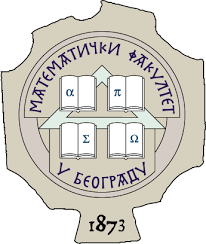
\includegraphics[width=0.3\textwidth]{matf_logo.png}
        
        \large{Београд, мај 2020}
        
    \end{center}
\end{titlepage}
\newpage
\pagenumbering{roman}
\tableofcontents

\newpage
\pagenumbering{arabic}
\section{Увод}
\label{sec:uvod}

\section{Ним}
\label{sec:nim}

Игра ним је игра са неколико гомила жетона за два играча. Број жетона и гомила је произвољан, тачније одређују их сами играчи. Играч који је на потезу може узети произвољан број жетона са једне гомиле, при чему мора узети бар један жетон и не сме узимати жетоне са више гомила. Играчи наизменично играју потезе. Постоје две варијанте игре: нормални и мизерни ним. У нормалном ниму побеђује играч који узме последњи жетон, док у мизерном губи играч који узме последњи жетон.

\begin{example}
На почетку партије на столу су три гомиле, са три, четири и пет жетона респективно. Партију играју два играча \textit{А} и \textit{Б}, \textit{А} игра први. 
\end{example}

Могући ток игре нормалног нима је приказан на слици \ref{fig:nimPrimer}.

\begin{figure}[H]
	\caption{Ток игре ним}
	\label{fig:nimPrimer}
	\begin{center}
		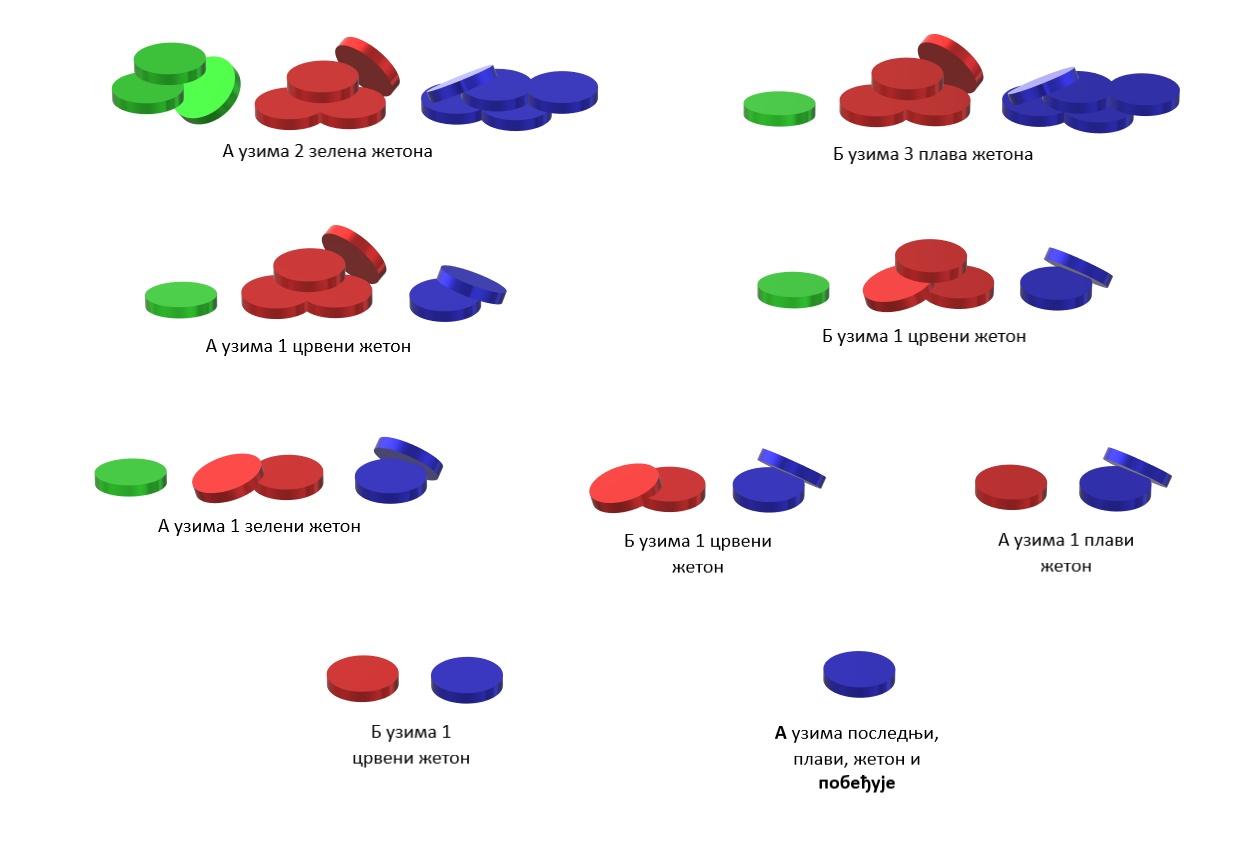
\includegraphics[width=\textwidth]{NimPrimer.png}
	\end{center}
\end{figure}

У општем случају, уколико се на столу налазе две гомиле, у зависности од броја жетона могући су следећи исходи нормалног нима:

\begin{itemize}
	\item На столу су две гомиле са по једним жетоном. Први играч мора да узме бар један жетон, чиме оставља другом играчу да узме последњи жетон и победи. У овој ситуацији очигледно је да \textbf{први играч гарантовано губи}.
	
	\item На столу су две гомиле, на првој један жетон, на другој два жетона. \textbf{Први играч има победничку стратегију}: уколико узме један жетон са гомиле где су два жетона (на слици \ref{fig:nimPrimer} узима 1 плави жетон), оставља следећем играчу две гомиле са по једним жетоном, што је за њега, као што смо видели, изгубљена позиција.
	
	\item На столу су две гомиле са по два жетона. Прва могућност јесте да први играч узме све са једне гомиле, чиме други играч истим тим потезом, узимајући све жетоне са друге гомиле побеђује. Друга могућност је да први играч узме један жетон, тако да је следеће стање игре заправо стање из претходног примера, у коме играч који је на потезу може да победи. У овој ситуацији \textbf{први играч губи} уколико други играч зна како да игра ним.
\end{itemize}

Сада би требало да је јасно да у овој игри нема среће, односно да је свака позиција победничка или изгубљена за играча који је на потезу. Амерички математичар Чарлс Бутон (енг. {~\em Charles Bouton}) је извршио комплетну математичку анализу игре 1902. године, односно одредио је све победничке и изгубљене позиције \cite{carls_buton}. Идеја је да се бројеви жетона на свакој гомили запишу у бинарном бројном систему, а затим се примени ексклузивна дисјункција (XOR) бит по бит, тј бинарна сума без преноса. 


\begin{example} 
	Нека су на столу дате две гомиле са три и четири жетона, тада је њихова бинарна сума без преноса:
	
	\begin{align*}
		3&		& 0 1 1&\\
		+4&		& 1 0 0&\\
		--&		&------&\\
		7&		& 1 1 1&
	\end{align*}
	
\end{example}

\begin{theorem}
	\label{thm:pobeda}
	У нормалном ниму, гарантовано ће победник бити играч након чијег потеза је бинарна сума без преноса жетона на свим гомилама једнака нула.
\end{theorem}

\begin{proof}
	Нека играч \textit{А} игра први, играч \textit{Б} други. На столу je $ n $ гомила са редом $ x_{1}, x_{2}, ... , x_{n} $ жетона, и нека је $ s $ ексклузивна дисјункција: 
	
	\begin{displaymath}
		s = x_{1} \oplus x_{2} \oplus x_{3} \ldots \oplus x_{n}.
	\end{displaymath}
	
	Након што играч \textit{А} одигра свој потез, $ t $ је ексклузивна дисјункција жетона:
	
	\begin{displaymath}
		t = y_{1} \oplus y_{2} \oplus y_{3} \ldots \oplus y_{n}.
	\end{displaymath}
	
	 Уколико је $ s = 0 $, како се жетони могу узети само са једне гомиле онда је $ x_{k} \neq y_{k} $ и $ x_{i} = y_{i} $ за $ i \neq k $, стога је:
	 
	 \begin{eqnarray*}
	 	t &=& 0 \oplus t \\
		  &=& s \oplus s \oplus t \\
		  &=& s \oplus (x_{1} \oplus x_{2} \oplus x_{3} ... \oplus x_{n}) \oplus (y_{1} \oplus y_{2} \oplus y_{3} ... \oplus y_{n}) \\
		  &=& s \oplus (x_{1} \oplus y_{1}) \oplus (x_{2} \oplus y_{2}) \oplus  \ldots \oplus (x_{n} + y_{n}) \\
		  &=& s \oplus (x_{k} \oplus y_{k}). 		 
	 \end{eqnarray*}
	 
	 Уколико је $ s = 0 $, онда је $ t \neq 0 $ јер важи $ x_{k} \neq y_{k} $ и $ x_{k} \oplus y_{k} $ никад неће бити нула. Овим је доказано да уколико је тренутна бинарна сума без преноса нула, шта год противник одиграо сума ће бити различита од нула.
	 
	 Уколико je $ s \neq 0 $, нека је $ d $ позиција бита највеће тежине у $ s $ и нека је $ x_{k} $ гомила у којој је бит највеће тежине такође на позицији $ d $, овакав бит увек постоји, јер бит највеће тежине из $ s $ долази од бита највеће тежине неких од гомила са $ x_{1}, x_{2}, ... , x_{n} $ жетона. У овом случају са гомиле $ x_{k} $ узима се $ x_{k} - y_{k} $ жетона, где је $ y_{k} = s \oplus x_{k} $, тако да је бинарна сума без преноса:
	 
	 \begin{eqnarray*}
	 	t &=& s \oplus x_{k} \oplus y_{k} \\ 
	 	&=& s \oplus x_{k} \oplus s \oplus x_{k} \\
	 	&=& s \oplus s \oplus x_{k} \oplus x_{k} \\
	 	&=& 0		 
	 \end{eqnarray*}
	 
	 Овим је доказано да уколико тренутна бинарна сума без преноса није нула, увек је могуће направити потез тако да бинарна сума без преноса буде нула.
	 
\end{proof}

За мизерни ним се може пратити иста стратегија као у теореми \ref{thm:pobeda} све док не остану само гомиле са по једним жетоном. Тада је победа гарантована ако играч који је на потезу остави непаран број гомила са по једним жетоном.

\begin{example} 
	Нека су на столу дате три гомиле са седам, пет, дванаест жетона. Играч \textit{А} игра први, играч \textit{Б} игра други.
	
	\begin{align*}
		7&		&   1 1 1&\\
		5&		&   1 0 1&\\
		+12&	& 1 1 0 0&\\
		---&	&--------&\\
		24&		& 1 1 1 0
	\end{align*}
		
	У $ 1 1 1 0 $ бит највеће тежине је на позицији три, тако да играч \textit{А} узима са треће гомиле $ 1 1 0 0 - (1 1 0 0 \oplus  1 1 1 0) = 12 - 2 = 10 $  жетона.	
	
	\begin{align*}
		7&		&  	1 1 1&\\
		5&		&   1 0 1&\\
		+2&		&  	  1 0&\\
		---&	&--------&\\
		14&		&   0 0 0
	\end{align*}
	
	\textit{Б} узима  са друге гомиле два жетона.
	
	\begin{align*}
		7&		&   1 1 1&\\
		3&		&     1 1&\\
		+2&		&  	  1 0&\\
		---&	&--------&\\
		12&		&   1 1 0
	\end{align*}
	
	\textit{А} узима са прве гомиле шест жетона.
	
	\begin{align*}
		1&		&       1&\\
		3&		&     1 1&\\
		+2&		&  	  1 0&\\
		---&	&--------&\\
		6&		&     0 0
	\end{align*}
	
	\textit{Б} узима са треће гомиле један жетон.
	
	\begin{align*}
		1&		&       1&\\
		3&		&     1 1&\\
		+1&		&  	  	1&\\
		---&	&--------&\\
		5&		&     1 1
	\end{align*}
	
	\textit{А} узима са друге гомиле три жетона.
	
	\begin{align*}
		1&		&       1&\\
		+1&		&  	  	1&\\
		---&	&--------&\\
		2&		&       0
	\end{align*}
	
	\textit{Б} узима са прве гомиле један жетона.
	
	\begin{align*}
		1&		&  	  	1&\\
		---&	&--------&\\
		1&		&       1
	\end{align*}
	
	\textit{А} узима последњи жетон и побеђује.
	
\end{example}

\subsection{Варијане игре ним}
\label{subsec:varijante_igre_nim}

Постоје многе варијанте нима \cite{nimvariants}, које се од оригиналне верзије углавном разликују по томе што садрже бар једно додатно правило за игру. Неке од варијанти су:
\begin{itemize}
	\item \textbf{Индекс k игра} (енг. {~\em Index-k nim}) у којој је дозвољено да играч у једном потезу узме жетоне са више гомила. 
	\item \textbf{Грандијева игра} (енг. {~\em Grundy's game}) се игра са једном гомилом жетона, где је једини дозвољен потез дељење текуће гомиле на две гомиле са различитим бројем жетона. Игра се завршава када остану гомиле са два или мање жетона.
	\item \textbf{Похлепни ним} (енг. {~em Greedy nim}) у којој је дозвољено узимање жетона само са најбројније гомиле, а уколико је више таквих гомила онда је дозвољено узимање са произвољне најбројније гомиле.
	\item \textbf{Градитељски ним} (енг. {~\em Building nim}) која се игра у две фазе. У првој фази играчи наизменично на $ n $ гомила распоређују $ p $ жетона, прво на гомиле без елемената, ова фаза се завршава када се распореде сви жетони. У другој фази се игра нормални ним. 
	\item \textbf{Витховофа игра} (енг. {~\em Wythoff's game}) \cite{wythoff1907modification} се игра са две гомиле жетона; играчи наизменично узимају жетоне са једне или обе гомиле. Приликом узимања жетона са обе гомилe, рецимо $ k (> 0) $ са једне и $ l (> 0) $ са друге, мора да буде испуњен услов $ |k - l| < a $, где је $ a $ задати позитиван број који се одређује пре почетка партије и не мења се у току саме партије. Игра се завршава када број жетона на столу буде нула, а онај играч који је уклонио последњи жетон или жетоне је победник. Сваки играч када је на потезу мора да уклони бар један жетон. У класичној Витхоф игри $ a $ je $ 1 $, што значи да ако играч узима жетоне са обе гомиле, број узетих жетона мора бити једнак. Игра се еквивалентно може описати и као игра са краљицом на шаховској табли: негде на шаховској табли је краљица, играч који је на потезу може да помери краљицу произвољан број корака у правцу југа, запада, или југозапада. Победник је играч који први помери краљицу у доњи леви угао табле \cite{cut-the-knot, singingbanana-youtube}. Забележено је да се ова игра играла у Кини  под именом "\begin{CJK}{UTF8}{gbsn}捡石子\end{CJK} jiǎn shízǐ", односно енг. {~\em picking stones} \cite{Yaglom}. Холандски математичар В. А. Витхоф ({~\em W. A. Wythoff}) је 1907. године објавио математичку анализу ове игре. \cite{wythoff1907modification}
\end{itemize}

\section{Оптимална стратегија}
\label{sec:optimalna_strategija}

Све позиције се елементарно могу одредити типови позиција, било која позиција се може представити паром бројева $ (x, y) $, где је $ x \le  y $. Овде  $ x $ и $ y $ представљају бројеве жетона на две гомиле или координате позиције краљице (при чему су координате доњег левог угла (0, 0)). Све могуће позиције могу се разврстати у две категорије, добијене и изгубљене. 

\begin{definition}
	У изгубљеној позицји, играч који је на потезу губи ако противник игра како треба, другим речима наредни играч може да победи шта год одиграо противник. У добијеној позицији, играч који је на потезу побеђује ако игра како треба.
\end{definition}

Класификација позиција на добијене и изгубљене се дефинише рекурзивно на следећи начин:
\begin{enumerate}
	\item $ (0, 0) $ је по дефиницији изгубљена позиција јер играч који је на потезу не може да одигра ниједан валидан потез, па је његов противник победник.
	\item Било која позиција из које је у једном потезу достижна изгубљена позиција је добијена позиција.
	\item Ако сваки потез води ка некој добијеној позицији, онда је то изгубљена позиција.
\end{enumerate}

\textit{Jasno je da je pozicija (x,x) dobijena ako je x>0. Dalje,  ako su (x',y'), x'<y', i (x'',y''), x''<y'', dve izgubljene pozicije, onda je $\{x',y'\} \cap   \{x'',y''\}= \emptyset $:
ako je npr. y'=x'', onda se iz izgubljene pozicije (x'',y'') skidanjem sa jedne gomile moze doci u poziciju
(y''-(y''-x'),x'')=(x',y') koja je izgubljena za protivnika, sto je kontradikcija.}

Да би се Витхофова игра ирала на најбољи могући начин, потребно је знати две ствари:
\begin{itemize}
	\item Препознати природу тренутне позиције, да ли је добијена или изгубљена.
	\item Уколико је тренутна позиција добијена, треба одредити следећи потез тако да се противник нађе у изгубљеној позицији.
\end{itemize}

Класификација позиција на добијене и изгубљене је важна, јер ако је тренутна позиција добијена, постоји потез који води ка изгубљеној позицији, а тај потез се може одредити и победити. Са друге стране ако је тренутна позиција изгубљена не може се урадити ништа, само одиграти произвољан валидан потез и надати се да ће противник да одигра погрешан потез, с обзиром на то да се у једном потезу са изгубљене позиције стиже на добијену позицију, са које противник може да победи ако зна да одреди изгубљену позицију. 

\begin{example}
	За $ a = 1 $, позиција $ (1, 2) $ је изгубљена позиција, зато што су са ње у једном потезу достижне само позиције $ (0, 1), (0, 2), (1, 0) $ и $ (1, 1) $, које су добијене позиције. Још неке изгубљене позиције приказане су у табели \ref{tab:a_1_Ppozicije} и на слици \ref{fig:p_positions_a=1} црвена поља су добијене позиције. 
\end{example}
	
\begin{table}[h!]
	\caption{Приказ првих $ 10 $ изгубљених $ (A, B) $ позиција за $ a = 1 $}
	\label{tab:a_1_Ppozicije}
	\begin{center}
		\begin{tabular}{  c | c | c }
			{\textbf{n}} &  {\textbf{A}} &  {\textbf{B}} \\
			\hline
			0 & 0 & 0 \\
			1 & 1 & 2 \\
			2 & 3 & 5 \\
			3 & 4 & 7 \\
			4 & 6 & 10 \\
			5 & 8 & 13 \\
			6 & 9 & 15 \\
			7 & 11 & 18 \\
			8 & 12 & 20 \\
			9 & 14 & 23 \\
			10 & 16 & 26\\ 
		\end{tabular}
	\end{center}
\end{table}

\begin{figure}[H]
	\caption{Визуелни приказ изгубљених позиција за $ a = 1 $}
	\label{fig:p_positions_a=1}
	\begin{center}
		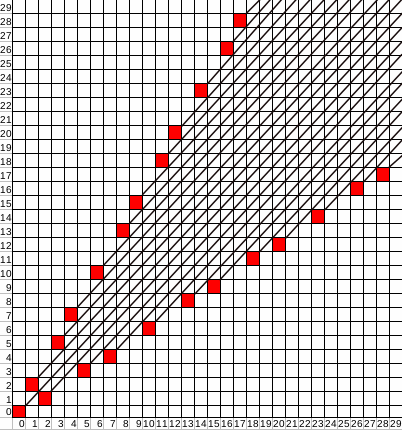
\includegraphics[width=350px, height=350px]{p_positions_a=1.png}
	\end{center}
\end{figure}

\begin{example}
	За $ a = 2 $, изгубљене позиције приказане су у табели \ref{tab:a_2_Ppozicije} и на слици \ref{fig:p_positions_a=2} црвена поља су добијене позиције.
\end{example}

\begin{table}[h!]
	\caption{Приказ првих $ 10 $ изгубљених $ (A, B) $ позиција за $ a = 2 $}
	\label{tab:a_2_Ppozicije}
	\begin{center}
		\begin{tabular}{  c | c | c }
			{\textbf{n}} &  {\textbf{A}} &  {\textbf{B}} \\
			\hline
			0 & 0 & 0 \\
			1 & 1 & 3 \\
			2 & 2 & 6 \\
			3 & 4 & 10 \\
			4 & 5 & 13 \\
			5 & 7 & 17 \\
			6 & 8 & 20 \\
			7 & 9 & 23 \\
			8 & 11 & 27 \\
			9 & 12 & 30 \\
			10 & 14 & 34\\ 
		\end{tabular}
	\end{center}
\end{table}

\begin{figure}[H]
	\caption{Визуелни приказ изгубљених позиција за $ a = 2 $}
	\label{fig:p_positions_a=1}
	\begin{center}
		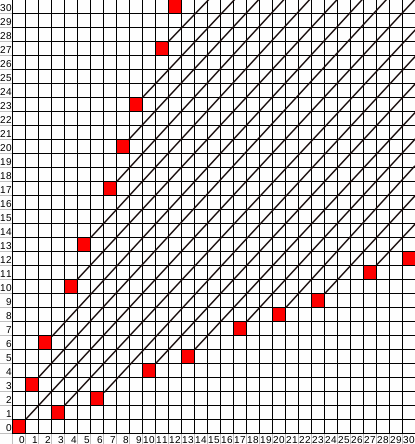
\includegraphics[width=350px, height=350px]{p_positions_a=2.png}
	\end{center}
\end{figure}

\begin{example}
	На столу је табела $ 10x10 $, на позицији $ (0, 0) $ је циљ. Игру играју два играча \textit{А} и \textit{Б}, померајући наизменично краљицу од почетне позиције $ (x,y) $. Дозвољено је краљицу померати ка југу, југозападу и западу у односу на текућу позицију.  Победник је играч који први доведе краљицу до циља. На табли су све позиције $ (x, y) $, а не само $ x \leq y $.
	
	Играч \textit{А} игра први, \textit{Б} други. На слици \ref{fig:sahovska_tabla_pozicije_a_2} је дат приказ изгубљених позиција(зелена поља) и како се до њих може доћи (плаве и црвене стрелецие). Уколико је краљица на позицији $ (0, y), (x,0) $ или $ (x,x) $, при чему је $ x > 0, y > 0 $, играч \textit{А} уколико игра како треба у једном потезу може довести краљицу до циља и победити. Уопште, уколико је краљица на позицији, из које се плавом или црвеном стрелицом може прећи у зелено поље, играч \textit{А} може краљицу једним потезом довести до изгубљене позиције, са које су достижне само добијене позиције и са којих играч \textit{А} може директно довести краљицу до циља или је померити на неку од преосталих изгубљених позција ближих циљу. Уколико из тренутне позиције ниједан валидан потез не води до зеленог поља, онда је та позиција изгубљена. 
	
	Са позиције $ (4, 9) $ може се доћи само на позиције покривене плавим или црвеним стрелицама. Због тога је та позиција изгубљена.
\end{example}
 
\begin{figure}[H]
	\caption{Приказ изгубљених позиција на табли $ 10x10 $ за $ a = 2 $}
	\label{fig:sahovska_tabla_pozicije_a_2}
	\begin{center}
		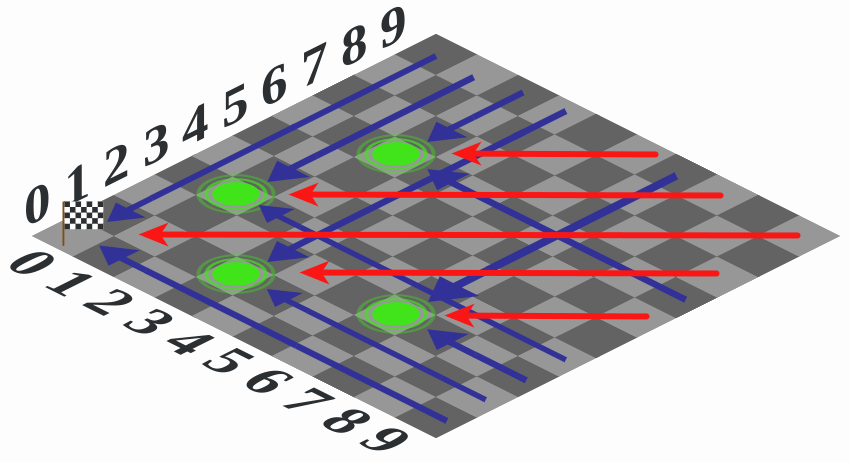
\includegraphics[width=\textwidth]{10x10.png}
	\end{center}
\end{figure}

Свака позиција је добијена или изгубљена, лако се види како се, корак по корак, за сваку позицију може установити тип. У наставку следи приказ три начина да се одреде типови свих позиција: рекурзивна, алгебарска или аритметичка стратегија \cite{10.2307/2321643}.

\subsection{Рекурзивна стратегија}

Рекурзивни поступак за одређивање изгубљених позиција заснива се на оператору $ \mex $.

\begin{definition}
	\label{def:mex}
	$\mex(A)$ означава најмањи природни број који није у скупу $ A $, тј. $ \mex(\emptyset)=0 $ и
$ \mex(A)=\min\{i | i\notin A\} $.
\end{definition}

Описани начин добијања изгубљених позиција $ (A_{n}, B_{n}) $, може се поједноставити, што показује следећа теорема. 

\begin{theorem} [Рекурзивна карактеризација изгубљених позиција]
	\label{thm:reukrzivna_strategija}
	Нека је 
	\begin{eqnarray}
		&A_{n} = &\mex \{ A_{i}, B_{i} : i < n \}\\
		&B_{n} = &A_{n} + an
	\end{eqnarray}
	Тада је скуп свих изгубљених позиција
	$ P = \cup_{i=0}^{\infty} \{(A_{i},B_{i})\} $.
\end{theorem}

\begin{proof}
	
	Из дефиниција $ A_{n} $ и $ B_{n} $ датих у теореми важи да ако је $ A = \cup_{n=1}^{\infty} A_{n} $ и  $ B = \cup_{n=1}^{\infty} B_{n} $ онда су $ A_{n} $ и $ B_{n} $ \textbf{комплементарни} скупови, тако да је $ A \cup B = Z^{+} $ скуп целих позитивних бројева  и $ A \cap B = \emptyset $. 
	$ A \cup B = Z^{+} $ важи јер због дефиниције \ref{def:mex} ниједан број не може бити испуштен, а $ A \cap B = \emptyset $ јер у случају да је $ A_{n} = B_{m} $, и $ n > m $, следи да је $ A_{n} $ $ \mex $ скупа који садржи $ B_{m} = A_{n} $ што је у супротности са дефиницијом \ref{def:mex}. Случај када је $ n \leq m $ је немогућ јер је тада $ B_{m} = A_{m} + am \geq  A_{n} + an > A_{n} $. 
	
	Да би се доказала теорема остаје да се докаже да се из неке позиције $ (A_{n}, B_{n}) $ не може доћи у неку претходну позицију $ (A_{i}, B{i}), i < n $, и да се из ове позиције једним потезом може прећи само у (за противника) добијене позиције.
	
	Из изгубљене позицицје, једним потезом може се прећи само у добијену позицију. Из позиције $ (A_{n}, B_{n}) $ узимањем жетона само са једне гомиле прелази се у другу позицију, нова позиција не може бити облика $ (A_{i}, B_{i}) $. Ово следи из чињенице да су  $ A_{n} $ и $ B_{n} $ комплементарни скупови. Уколико узима жетоне са обе гомиле такође прелази у позицију која није облика $ (A_{i}, B_{i}) $. У противном би за нову позицију $ (A_{i}, B_{i}) $, морало би да важи $ |(B_{n} - B_{i}) - (A_{n}-A_{i})| < a $. Међутим из једнакости $ B_{n} - A_{n} = an $ следи $ |(n-i)a| < a $, што је тачно само ако је $ i = n $, што је контрадикција. 
	
	Из добијене позиције, једним потезом може се прећи у изгубљену позицију.
	Размотримо позиције у које се може прећи из позиције $ (x, y), x \le y $ која није облика $ (A_{i}, B_{i}), i \ge 0 $. Како су $ A_{n} $ и $ B_{n} $ комплементарни скупови, може се сматрати да је $ x = B_{n} $, или је $ x = A_{n} $, за неко $ n \ge 0 $ .
	\begin{itemize}
		\item \label{case:slucaj1} Случај 1: Ако је $ x = B_{n} $ онда се из позиције $ (x = B_{n}, y) $ може једним потезом прећи у изгубљену позицију $ (A_{n}, B_{n}) $ 
		\item \label{case:slucaj2} Случај 2: Ако је $ x = A_{n} $ и $ y > B_{n} $, онда се смањивањем $ y $ може доћи у позицију $ (A_{n}, B_{n}) $. У противном, ако је $ A_{n} \le y < B_{n} $ онда се смањивањем $ x $ и $ y $ може прећи у позицију $ (A_{m}, B_{m}) $, где је $ m = \lfloor \frac{d}{a} \rfloor $ и $ d = y - x $. Заиста, из $ d = y - A_{n} < B_{n} - A_{n} = an $, следи да је  $ m = \lfloor \frac{d}{a} \rfloor \le \frac{d}{a} < n $. Поред тога важи неједнакост $ y = A_{n} + d \ge A_{m} + am = B_m $. Из позиције $ (x, y) $ смањивањем обе компоненте прелази се у позицију $ (A_{m}, B_{m}) $, при чему за смањење компоненти важи неједнакост $ |(y - B_{m}) - (x - A_{m})| = d - am < a $.
	\end{itemize}
	
\end{proof}

\textbf{primer - objasnjenje dobijanja nekoliko brojeva u tabeli 2.}

\textbf{Objasnjenje sta je strategija igre iz rada, dosta je dobra. Malo se prekalapa sa prethodnim, pa je potrebno uskladjivanje.
}

\textbf{Ocena slozenosti $ O(\log x) $ za odredjivanje poteza iz pozicije (x,y)}

\subsection{Алгебарска стратегија}

Изгубљене позиције $ (A_{n}, B_{n}) $ могу се експлицитно изразити на следећи једноставан начин $ A_{n} = \lfloor \alpha n \rfloor, B_{n} = \lfloor \beta n \rfloor $, где је:

\begin{eqnarray}
	&\alpha = &\frac{2 - a + \sqrt{a^2 + 4}}{2} \label{def:alpha}\\  
	&\beta = &\alpha + a \label{def:beta}
\end{eqnarray}

Овде су $ \alpha $ и $ \beta $ ирационални за свако $ a > 0 $, и $ \alpha $ је позитиван корен једначине $ \alpha^{-1} + \beta^{-1} = 1 $. Из ове једнакости следе неједнакости:
$ 1<\alpha<2 $: због $ \beta^{-1} = (\alpha+a)^{-1} < \frac{1}{2 }$ мора да буде $ \alpha^{-1} > \frac{1}{2} $.

Ако је $ \alpha $ произвољан ирационални број, онда се целобројни растућии низ $ (\lfloor \alpha 0 \rfloor, \lfloor \alpha 1 \rfloor, ... \lfloor \alpha n \rfloor) $ зове Бетијев низ (енг. {~\em Beatty}), где $ i = 0...n $.

Најпре следи доказ општег тврђења о Бетијевим низовима.

\begin{lemma}
	Нека су $ \alpha $ и $ \beta $ позитивни ирационални бројеви који задовољавају $ \alpha^{-1} + \beta^{-1} = 1 $ и нека је 
	\begin{eqnarray*} 
		&A_{n}^{'} = &\lfloor \alpha n \rfloor\\
		&B_{n}^{'} = &\lfloor \beta n \rfloor\\
		&A^{'} = &\cup_{n=1}^{\infty}\{A_{n}^{'}\}\\
		&B^{'} = &\cup_{n=1}^{\infty}\{B_{n}^{'}\}
	\end{eqnarray*}
	Тада су $ A^{'} $ и $ B^{'} $ комплементарни Беатијеви низови.
\end{lemma}

\begin{proof}
	Довољно је показати да се тачно један елемент уније $ A_{n}^{'} \cup B_{n}^{'} $ налази у интервалу $ [N,N+1) $, за сваки позитиван број $ N $, тј. довољно је да одредимо колико има бројева из скупа $ A_{n}^{'} \cup B_{n}^{'} $ који су мањи од $ N $, ако је $ N > 1 $.
	
	Бројева из $ A_{n}^{'} $ мањих од $ N $ има $ \lfloor \frac{N}{\alpha} \rfloor $.
	
	Бројева из $ B_{n}^{'} $ мањих од $ N $ има $ \lfloor \frac{N}{\beta} \rfloor $.
	
	Сабирањем двоструких неједнакости:
		\begin{eqnarray*}
			&\frac{N}{\alpha} - 1 < \lfloor \frac{N}{\alpha} \rfloor < \frac{N}{\alpha}\\
			&\frac{N}{\beta} - 1 < \lfloor \frac{N}{\beta} \rfloor < \frac{N}{\beta}
		\end{eqnarray*}
	
	добија се:
		\begin{displaymath}
		N - 2 < \lfloor \frac{N}{\alpha} \rfloor + \lfloor \frac{N}{\beta} \rfloor < N
		\end{displaymath} 
	
	Oдавде следи да је $ \lfloor \frac{N}{\alpha} \rfloor + \lfloor \frac{N}{\beta} \rfloor = N - 1 $, тј. $ N - 1 $ бројева из уније $ A_{n}^{'} \cup B_{n}^{'} $ је мање од $ N $. Слично важи и да је $ N $ бројева из $ A_{n}^{'} \cup B_{n}^{'} $ мање од $ N + 1 $. Према томе, тачно $ N - (N - 1) = 1 $ елемент те уније припада интервалу $ [N,N+1) $ и нема дупликата.
\end{proof}

\begin{lemma}
	\label{lemma:n}
	$ n = \lfloor \frac{(x+1)}{\alpha} \rfloor $
	(ovo sledi iz dvostruke nejednakosti
	$\frac{x}{\alpha}<n<\frac{x+1}{\alpha}$
	zbog toga sto je razlika
	$\frac{x+1}{\alpha}-\frac{x}{\alpha}<1$,
	a interval duzine manje od 1 moze da sadrzi najvise jedan celi broj)
\end{lemma}


\begin{lemma}[Алгебарска карактеризација изгубљених позиција] Нека су $ \alpha $ и $ \beta $ дефинисани једнакостима \eqref{def:alpha}, \eqref{def:beta}. Тада је скуп свих изгубљених позиција $ P = \cup_{n=0}^{\infty} \{(\lfloor \alpha n \rfloor, \lfloor \beta n \rfloor)\} $.
\end{lemma}

\begin{proof}
	Уочимо да је $ A'_{0} = 0, B'_{0} = 0 $ и $ B'_{n} - A'_{n} = an $. Такође како су $ A'_{n} $ и $ B'_{n} $ растући и комплементарни низови, важи још и да је $ A'_{n} = \mex \{ A'_{i}, B'_{i} : i < n \} $. Из ове чињенице индукцијом следи да је $ A'_{n} = A_{n} $ и $ B'_{n} = B_{n}  $ за $ n \ge 0 $.
\end{proof}

Нека је $ (x, y), x \leq y $ тренутна позиција игре. Тада је $ x = \lfloor n \alpha \rfloor = A_{n} $, где је $ n = \lfloor \frac{(x+1)}{\alpha} \rfloor $ или је $ x = \lfloor n \beta \rfloor = B_{n} $, где је $ n = \lfloor \frac{(x+1)}{\beta} \rfloor $, видети доказ теореме \ref{thm:reukrzivna_strategija} и леме \ref{lemma:n}. На пример, ако је $ x = \lfloor n \alpha \rfloor = A_{n} $, и $ \lfloor n \alpha \rfloor < y < \lfloor n \beta \rfloor $ онда се смањивањем $ x $ и $ y $ може прећи у позицију $ (\lfloor m \alpha \rfloor, \lfloor m \beta \rfloor) $, где је $ m = \lfloor \frac{d}{a} \rfloor $ и $ d = y - x $, при чему за смањење компоненти важи неједнакост $ |(y - \lfloor m \beta \rfloor) - (x - \lfloor m \alpha \rfloor)| = d - am < a $.

\begin{example}
	У специјалном случају за $ a = 1 $ важи $ \alpha = \frac{1 + \sqrt{5}}{2} $, што је златни пресек.
	
	Низ $ \lfloor \alpha n \rfloor $ се назива доњи Витхофов низ ($ A_{n} $):
	$ 1, 3, 4, 6, 8, 9, 11, 12, 14, 16 \ldots $. Низ $ \lfloor (\alpha + 1) n \rfloor $ се назива горњи Витхофов низ ($ B_{n} $):
	$ 2, 5, 7, 10, 13, 15, 18, 20, 23, 26 \ldots $
\end{example}

\subsection{Аритметичка стратегија}

Сваки ирационални број се једнозначно може представити бесконачним верижним разломком. Нека је $ \alpha $ ирационалан број који се може једнозначно представити бесконачним верижним разломком облика:

\begin{displaymath}
	\alpha = a_{0} + \frac{1}{a_{1} + \frac{1}{a_{2} + \frac{1}{a_{3} + ...}}},
\end{displaymath}

односно,

\begin{displaymath}
	\alpha = \lim\limits_{n \rightarrow \infty} [a_{0}, a_{1}, a_{2}, a_{3}, ...].
\end{displaymath}

Чланови низа $ a_{n} $ добијају се поступком сличним Еуклидовом алгоритму, тј. број $ \alpha $ одређује низ $ a_{n} $. Обрнуто сваки бесконачни верижни развoј једнозначно одређује ирационални број. При томе, ако је $ n > 1 $, онда је $ a_{n} > 1 $.

Рационални бројеви $ a_{0}, a_{0} + \frac{1}{a_{1}}, a_{0} + \frac{1}{a_{1} + \frac{1}{a_{2}}}, a_{0} + \frac{1}{a{1} + \frac{1}{a_{2} + \frac{1}{a_{3}}}} $ где је $ a_{i} > 0 $ и $ i > 0 $ су конвергенти броја $ \alpha $. 

Конвергенти су веома добре рационалне апроксимације $ \alpha $. Показује се да ако је $ \alpha $ ирационалан и $ |\alpha - \frac{p_{n}}{q_{n}}| < \frac{1}{2q_{n}^2} $, где су $ p_{n} $ и $ q_{n} $ узајамно прости, онда је $ \frac{p_{n}}{q_{n}} $ увек конвергент $ \alpha $.

\begin{displaymath}
\frac{p_{n}}{q_{n}} = [1, a_{1}, , a_{2}, , a_{3}, ..., a_{n}]
\end{displaymath}

\begin{lemma}
	\label{def:p_q_nizovi}
	$ p $ и $ q $ су низови рекурзивно дефинисани на следећи начин:
	
	\begin{eqnarray}
	p_{-1} = 1, p_{0} = a_{0}, p_{n} = a_{n}p_{n-1} + p_{n-2}, (n \geq 1 )\\
	q_{-1} = 0, q_{0} = 1, q_{n} = a_{n}q_{n-1} + q_{n-2}, (n \geq 1 ).
	\end{eqnarray}
	
	где је $ a_{0}, a_{1}, ... $ јединствени бесконачни низ природних бројева за које важи $ a_{0} = 1 $ и $ a_{1}, a_{2}, ... ,  $ су позитивни и $ a_{n} \ne 1 $.
\end{lemma}

\begin{proof}
	
	Индукцијом
	
	http://poincare.matf.bg.ac.rs/%7Eezivkovm//nastava/kripto.pdf
	strane 92-93
\end{proof}

%Уобичајени запис за бесконачни верижни разломак је:

%\begin{displaymath}
%	[a_{0}, a_{1}, a_{2}, a_{3}, ...].
%\end{displaymath}

%Сваки ирационални број се једнозначно може преставити бесконачним верижним разломком. где се чланови низа $ a_{i} $ добијају се поступком Еуклидовог алгоритма.

%\begin{eqnarray}
%	\alpha = 1 + \frac{1}{a_{1} + \frac{1}{a_{2} + \frac{1}{a_{3} + ...}}} = [1, a_{1}, a_{2}, a_{3}, ...] 
%\end{eqnarray}

%Чланови низа $ a_{n} $ добијају се поступком сличним Еуклидовом алгоритму, тј. број $ \alpha $ одређује низ $ a_{n} $. Обрнуто сваки бесконачни верижни развoј једнозначно одређује ирационални број. При томе, ако је $ n > 1 $, онда је $ a_{n} > 1 $.

%За $ \frac{p_{n}}{q_{n}} $, при чему су $ p_{n} $ и $ q_{n} $ узајамно прости, важи да је конвергент ирационалног броја $ \alpha $.  

%\begin{displaymath}
%	\frac{p_{n}}{q_{n}} = [1, a_{1}, , a_{2}, , a_{3}, ..., a_{n}]
%\end{displaymath}

%\begin{lemma}
%	\label{def:p_q_nizovi}
%	$ p $ и $ q $ су низови рекурзивно дефинисани на следећи начин:
%	
%	\begin{eqnarray}
%	p_{-1} = 1, p_{0} = a_{0}, p_{n} = a_{n}p_{n-1} + p_{n-2}, (n \geq 1 )\\
%	q_{-1} = 0, q_{0} = 1, q_{n} = a_{n}q_{n-1} + q_{n-2}, (n \geq 1 )
%	\end{eqnarray}
%	
%	где је $ a_{0}, a_{1}, ... $ јединствени бесконачни низ природних бројева за које важи $ a_{0} = 1 $ и $ a_{1}, a_{2}, ... ,  $ су позитивни и $ a_{n} \ne 1 $.
%\end{lemma}
%
%\begin{proof}
%		http://poincare.matf.bg.ac.rs/%7Eezivkovm//nastava/kripto.pdf
%strane 92-93
%\end{proof}


. Нека је $ \alpha $ ирационалан број, који задовоља услов $ 1 < \alpha < 2 $. Број  $ \alpha $ може се једнозначно представити бесконачним верижним разломком:

Specijalno, verizni razvoj broja $ \alpha $ definisanog jednakoscu \eqref{3} je
[1,a,a,a,a...]

to bi mogla da bude lema. 

dokaz: predlazem da to dokazete direktno, prema postupku za odredjivanje veriznog razvoja. Da biste se bolje snasli, mozete da to uradite prvo za a=1, pa za a=2, pa onda za opsti slucaj. Naravo, u dokaz cete da stavite samo opsti slucaj.

// u radu u casopisu on moze da kaze da je nesto poznato. U mater radu vi te stvari morate da dokazete, ako nisu previse komplikovane; a nisu

Низ бројилаца $ p_{n} $ може се искористити као низ тежина за специјални бројни систем, за који кажемо да је $ p $-систем. Слично, низ именилаца $ q_{n} $ може се искористити као низ тежина за други бројни систем, за који кажемо да је $ q $-систем.

\begin{theorem}
	\label{thm:p_q_sistemi}
	У $ p $-систему се сваки позитиван природни број $ N $ јединствено може записати на следећи начин:
	
	\begin{eqnarray}
		\label{p_sistem} N = \sum_{i=0}^{m} s_{i}p_{i}, 0 \le s_{i} \le a_{i+1}
	\end{eqnarray}
	ако је $ s_{i+1} = a_{i+2} $ онда је $ s_{i} = 0  $ за свако $ i \ge 0 $.
	
	Слично важи и за $ q $-систем :
	
	\begin{eqnarray}
		\label{q_sistem} N = \sum_{i=0}^{n} t_{i}q_{i}, 0 \le t_{0} < a_{1}, 0 \le t_{i} \le a_{i+1}
	\end{eqnarray}
	ако је $ t_{i} = a_{i+1} $ онда је $ t_{i-1} = 0 $ за свако $ i \ge 1 $.
	
	Где су $ s_{i} $, односно $ t_{i} $ цифре броја $ N $  у $ p $-систему, односно $ q $-систему.
\end{theorem} 

\begin{proof}
	Дати број $ N $, где је $ m $ највећа вредност тако да је задовољено $ p_{m} \leq N $, може се разложити помоћу низа дељења са остатком на следећи начин:
	
	\begin{eqnarray*}
		&N = &s_{m}p_{m} + r_{m}, 0 \leq r_{m} < p_{m}\\
		&r_{m} = &s_{m-1}p_{m-1} + r_{m-1}, 0 \leq r_{m-1} < p_{m-1}\\
		& . \\
		& . \\
		& . \\
		&r_{i+1} = &s_{i}p_{i} + r_{i}, 0 \leq r_{i} < p_{i}\\
		& . \\
		& . \\
		& . \\
		&r_{2} =& s_{1}p_{1} + r_{1}, 0 \leq r_{1} < p_{1}\\
		&r_{1} =& s_{0}p_{0} 
	\end{eqnarray*}
	
	Другим речима, долази се до разлагања броја $ N $ у $ p $-систему 
	
		 \begin{eqnarray}
			 \label{razlaganje} N = \sum_{i=0}^{m} s_{i}p_{i} 
		 \end{eqnarray}
	
	Приметимо да разлагање ~\eqref{razlaganje} важи независно од тога какав је низ $ p_{0} = 1 < p_{1} < \ldots $. Специјално, ако је $ p_{i} = b^{i}, b > 1 $, онда је то уобичајена представа броја $ N $ у систему са основом $ b $.
	
	Цифре $ s_i $ у разлагању ~\eqref{razlaganje} задовољавају следеће услове:
	
	\begin{displaymath}
		s_{i} = \frac{r_{i+1} - r_{i}}{p_{i}} < \frac{r_{i+1}}{p_{i}} < \frac{p_{i+1}}{p_{i}} = \frac{a_{i+1}p_{i}+p_{i-1}}{p_{i}} = a_{i+1} + \frac{p_{i-1}}{p_{i}} \leq a_{i+1} + 1, 
	\end{displaymath} 
	 
	тако да је $ 0 \leq s_{i} \leq a_{i+1}, i \geq 0 $.
	
	
	Аналогне неједнакости $ 0 \le t_{i} \le a_{i+1} $ важе за $ i > 0 $. Међутим, за $ i = 0 $ због $ q_{-1} = 0 $ добија се:
	
	\begin{displaymath} 
		t_0=\frac{r_1-r_0}{q_0}\le \frac{r_1}{q_0} < \frac{q_1}{q_0}=
		\frac{a_1 q_0+q_{-1}}{q_0}=a_1,
	\end{displaymath}
	
	тј. важи строга неједнакост.
	
	Претпоставимо да је $ s_{i} = a_{i+1} $ и $ s_{i-1} \geq 1 $ онда је 
	\begin{displaymath}
		r_{i} = s_{i-1}p_{i-1} + r_{i-1} \geq p_{i-1} + r_{i-1} \geq p_{i-1},
	\end{displaymath}
	
	и даље
	
	\begin{displaymath}
		r_{i+1} = s_{i}p_{i} + r_{i} = a_{i+1}p_{i} + r_{i} = \geq a_{i+1}p_{i} + p_{i-1} \geq p_{i+1}
	\end{displaymath}
	
	што је контрадикција. Према томе, ако је $ s_{i} = a_{i+1} $ онда је $ s_{i-1} = 0 $ за свако $ i \ge 1 $
\end{proof}

\textbf{Ovde treba da dodate dokaz jedinstvenosti ovakve reprezentacije, to je bitna stvar.}

Приказ првих неколико бројева записаних у $ p $ и $ q $ систему, за $ a_{i} = 2 , i \ge 1 $ дат је у табели \ref{tab:p_q_sistem}.

\begin{table}[h!]
	\caption{Приказ првих неколико бројева записаних у $ p $ и $ q $ систему, за $ a_{i} = 2 , i \ge 1 $}
	\label{tab:p_q_sistem}
	\begin{center}
		\begin{tabular}{ | c | c | c | c | c  c | c | c | c | c | c |}
			\hline
			{$ \mathbf{q_{3}} $} &  {$ \mathbf{q_{2}} $} &  {$ \mathbf{q_{1}} $} &  {$ \mathbf{q_{0}} $} & & &  {$ \mathbf{p_{3}} $} &  {$ \mathbf{p_{2}} $} &  {$ \mathbf{p_{1}} $} &  {$ \mathbf{p_{0}} $} &\\
			12 & 5 & 2 & 1 & & & 17 & 7 & 3 & 1 &  {$ \mathbf{n} $}\\
			\hline
			&  &  & 1 & & &  &  &  & 1 & {$ \mathbf{1} $}\\
			&  & 1 & 0 & & &  &  &  & 2 & {$ \mathbf{2} $}\\
			&  & 1 & 1 & & &  &  & 1 & 0 &  {$ \mathbf{3} $}\\
			&  & 2 & 0 & & &  &  & 1 & 1 &  {$ \mathbf{4} $}\\
			& 1 & 0 & 0 & & &  &  & 1 & 2 &  {$ \mathbf{5} $}\\
			& 1 & 0 & 1 & & &  &  & 2 & 0 &  {$ \mathbf{6} $}\\
			& 1 & 1 & 0 & & &  & 1 & 0 & 0 &  {$ \mathbf{7} $}\\
			& 1 & 1 & 1 & & &  & 1 & 0 & 1 &  {$ \mathbf{8} $}\\
			& 1 & 2 & 0 & & &  & 1 & 0 & 2 &  {$ \mathbf{9} $}\\
			& 2 & 0 & 0 & & &  & 1 & 1 & 0 &  {$ \mathbf{10} $}\\
			& 2 & 0 & 1 & & &  & 1 & 1 & 1 &  {$ \mathbf{11} $}\\
			 1 & 0 & 0 & 0 & & & & 1 & 1 & 2 &  {$ \mathbf{12} $}\\
			 1 & 0 & 0 & 1 & & & & 1 & 2 & 0 &  {$ \mathbf{13} $}\\
			 1 & 0 & 1 & 0 & & & & 2 & 0 & 0 &  {$ \mathbf{14} $}\\
			 1 & 0 & 1 & 1 & & & & 2 & 0 & 1 &  {$ \mathbf{15} $}\\
			 1 & 0 & 2 & 0 & & & & 2 & 0 & 2 &  {$ \mathbf{16} $}\\
			 1 & 1 & 0 & 0 & & & 1 & 0 & 0 & 0 &  {$ \mathbf{17} $}\\
			\hline 
		\end{tabular}
	\end{center}
\end{table}

\begin{definition}
	Репрезентација $ R $ је  $ (m+1) $-торка за коју важи :

		\begin{eqnarray}
			R = (d_{m}, d_{m-1}, ... , d_{1}, d_{0}), 0 \le d_{i} \le a_{i+1}
		\end{eqnarray}

	ако је $ d_{i+1} = a_{i+2} $ онда је $ d_{i} = 0 $ за свако $ i \ge 0 $.

	Нека је 
	
		\begin{displaymath}
			I_{p} = \sum_{i=0}^{m} d_{i}p_{i}
		\end{displaymath} 		
	
	$ p $-интерпретација репрезентације $ R $. 
	
	Ако је $ d_{0} < a_{1} $, нека је 
	
		\begin{displaymath}
			I_{q} = \sum_{i=0}^{m} d_{i}q_{i}
		\end{displaymath}  
	
	$ q $-интерпретација репрезентације $ R $. 
	
	У супротном кажемо да не постоји $ q $-интерпретација $ R $.
	
	За сваки позитиван број $ k = \sum_{i=0}^{m} d_{i}p_{i} $ важи да је: 
	
		\begin{displaymath}
			R_{p}(k) = (d_{m}, d_{m-1}, ... , d_{1}, d_{0})
		\end{displaymath}
	
	$ p $-репрезентација $ R_{p}(k) $.
	
	Aко је $ d_{0} < a_{1} $ за сваки позитиван број $ k = \sum_{i=0}^{m} d_{i}q_{i} $ важи да је:
	
		\begin{displaymath}
			R_{q}(k) = (d_{m}, d_{m-1}, ... , d_{1}, d_{0})
		\end{displaymath}
	
	 $ q $-репрезентација $ R_{q}(k) $. 
	
	Веза између $ p $-интерпретације $ I_{p} $ и $ q $-репрезентације $ R_{q} $ је:
	
	\begin{displaymath}
		I_{p}(R_{q}(k)) = I_{p}(d_{m}, d_{m-1}, ..., d_{1}) = n
	\end{displaymath}
	
	Уколико у $ R $ померимо сваку цифру $ d_{i} $ у лево за једно место добијамо $ R' = (d_{m}, d_{m-1}, ... , d_{1}, d_{0}, 0) $, а уколико је $ R $ репрезентација са $ d_{0} = 0 $ онда када сваку цифру $ d_{i} $ померимо за једно место у десно добијамо $ R'' = (d_{m}, d_{m-1}, ... , d_{1}) $. 
\end{definition}

\begin{example}
	Број $ R_{q}(12) = 1000 $, а $ I_{p}(1000) = 17 $ (видети табелу \ref{tab:p_q_sistem}).
\end{example}

Описани $ p $ и $ q $ бројни системи могу се искористити за још један начин добијања изгубљених позиција, користећи следећа својства.

\begin{property}
	\label{prop:r_p_nule}
	Нека је $ n $ позитиван број. Уколико се репрезентација $ R_p(n) $ завршава парним бројем нула онда је $ n \in \{A_{k} | k>0\} $ идентична вредности из скупа $ A_{n} $, а ако се репрезентација $ R_p(n) $ завршава непарним бројем нула онда је $ n \in \{B_{k} | k>0\} $ идентичана вредности из скупа $ B_{n} $.
\end{property}

\begin{proof}
	TODO
\end{proof}

\begin{example}
	Посматрајући табеле \ref{tab:a_2_Ppozicije} и \ref{tab:p_q_sistem}, запажамо да се:
	\begin{itemize}
		\item $ R_{p}(3) = 10 $ се завршава са једном нулом (непаран број), па је $ 3 $ у низу $ B $, $ B_{1} = 3 $. 
		\item $ R_{p}(7) = 100 $ се завршава са две нуле (паран број), па је $ 7 $ у низу $ A $, $ A_{5} = 7 $.
		\item $ R_{p}(9) = 102 $ се завршава са нула нула (паран број), па је $ 9 $ у низу $ A $, $ A_{7} = 9 $.
	\end{itemize}
\end{example}

\begin{property}
	\label{prop:levi_pomeraj}

	За свако $ n \geq 1 $ $ p $ репрезентација броја $ B_{n} $ одговара левом померају $ p $ репрезентације $ 
	R_{p} $ броја  $ A_{n} $
	
		\begin{displaymath}
			R_{p} (B_{n}) = R_{p}^{'} (A_{n}) 
		\end{displaymath}

\end{property}

\begin{proof}
	TODO
\end{proof}

\begin{example}
	Нека је $ n = 3 $ тада је $ A_{3} = 4 $ и $ B_{3} = 10 $.
	
	\begin{alignat*}{3}
		R_{p}(B_{3}) &= R_{p}(10)	&=& 110,\\
		R_{p}(A_{3}) &= R_{p}(4)	&=& 11,\\
		R_{p}^{'}(A_{3}) &= 110,
	\end{alignat*}
	
	видетеи табеле \ref{tab:a_2_Ppozicije} и \ref{tab:p_q_sistem}.
\end{example}

\begin{property}
	\label{prop:r_q_nule}
	
	Нека је $ n $ позитиван број. Уколико се репрезентација $ R_q(n) $ завршава парним бројем нула онда је:

	\begin{displaymath}
		I_{p}(R_q(n)) = A_{n}
	\end{displaymath}

	Уколико се репрезентација $ R_q(n) $ завршава непарним бројем нула онда је: 
	
	\begin{displaymath}
		I_{p}(R_q(n)) = A_{n} + 1
	\end{displaymath}

\end{property}

\begin{proof}
	TODO
\end{proof}

\begin{example}
	Посматрајући табеле \ref{tab:a_2_Ppozicije} и \ref{tab:p_q_sistem}, запажамо да се:
	\begin{itemize}
		\item $ R_q(10) = 200 $ се завршава са две нуле (паран број), па је $ I_{p}(200) = 14 $, $ A_{10} = 14 $.
		\item $ R_q(7) = 110 $ се завршава са једном нулом (непаран број), па је $ I_{p}(110) = 10 $, $ A_{7} + 1 = 9 + 1 + 10  $.
	\end{itemize}
\end{example}

\textbf{Treba da dodate dokaze ovih svojstava. Ako nesto zapne, tu sam.}

На основу својстава \ref{prop:r_p_nule}, \ref{prop:levi_pomeraj} и \ref{prop:r_q_nule} може се извршити карактеризација текуће позиције и одредити следећи потез.

Претпоставимо да је текућа позиција $ (x, y), 0 < x \le y $. Најпре је потребно ирачунати $ R_{p}(x) $ и проверити да ли се завршава са парним или непарним бројем нула.

\begin{itemize}
	\item Уколико се $ R_{p}(x) $ завршава непарним бројем нула, онда је $ x = B_{n} $, тако да је победнички потез $ (x, y) \rightarrow (I_{p}(R''_{p}(x)), x) $.
	\item Уколико се $ R_{p}(x) $ завршава парним бројем нула, онда је $ x = A_{n} $. Ако је $ y > I_{p}(R'_{p}(x)) $ победнички потез је $ (x, y) \rightarrow (x, I_{p}(R'_{p}(x)) $. У противном, ако је $ y < I_{p}(R'_{p}(x) $, рачунамо $ d = y - x, m = \lfloor \frac{d}{a} \rfloor $. Уколико се $ R_{q}(m) $ завршава са парним бројем нула, онда је $ A_{m} = I_{p}(R_{q}(m)) $; у противном се завршава непарним бројем нула и $ A_{m} = I_{p}(R_{q}(m)) - 1 $. У оба случаја победнички потез је $ (x, y) \rightarrow (A_{m}, A_{m} + ma) $.
\end{itemize}

\section{Имплементација и евалуација}
\label{implementacija_evaluacija}

За сваку стратегију у табели \ref{tab:calculate_time_n} су приказани резилтати рачунања П табеле у милисекундама зависно од $ n $, при фиксном $ a = 2 $. 
За мерење је коришћена хроно библиотека (енг.{~\em chrono library}) \cite{chrono_library}. Сва мерења су извршена на раучунару са следећом конфигурацијом:
\begin{flushleft}
	CPU: Intel(R) Core(TM) i7-4510U CPU @ 2.00GHz\\
	RAM: Kingston 8GB 1600MHz DDR3\\
	OS: Debian GNU/Linux 9 (stretch)\\
	Compiler: gcc 6.3.0\\
\end{flushleft}

У табели \ref{tab:calculate_piles} приказана је зависност парова жетона у односу на $ n $ реда величине до $ 10^{31} $.

\subsection{Рекурзивна стратегија}

За раучунање П табеле рекурзивном стратегијом прво је потребно да израчунамо $ A_{i} $, тачније потребно је наћи $ mex $ (дефиниција (\ref{def:mex})). За тражење је коришћен помоћни низ димензије $ 2*n $, иницијализиван нулама. Тражење $ mex $-а  своди се на проналажење индекса прве нуле, с обзиром да за елементе $ A $ важи $ a <= 2*n $ сложеност у најгорем случају је $ O(n) $. Чиме је укупна временска сложеност конструкције П табеле $ O(n^2) $.\\

\lstinputlisting[language=C++, linerange={7-31}, caption=Рекурзивна стратегија рачунање П табеле]{./src/recursive.cpp}

\leavevmode\\
Графички приказ зависности $ n $ и времена у милисекундама дат је на слици \ref{fig:recursive}, за $ а = 2 $.

\begin{figure}[H]
	\caption{График рекурзивне стратегије за конструкцију П табеле}
	\label{fig:recursive}
	\begin{center}
		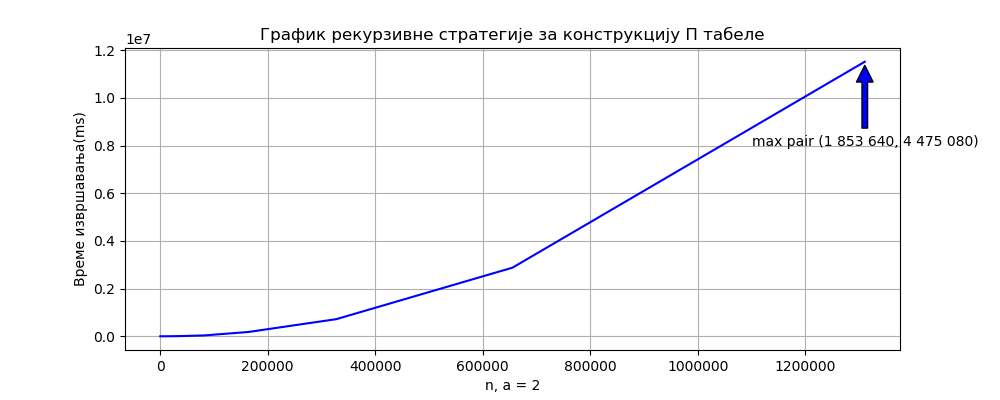
\includegraphics[width=\textwidth]{recursive.png}
	\end{center}
\end{figure}

\subsection{Алгебарска стратегија}

За разлику од рекурзиивне стратегије која користи имплицитну рекурзију, алгебарска стратегија користи експлицитну рекурзију, рачунајући $ alpha $ и $ beta $ (дефиниција (\ref{def:alpha_beta})). Чиме је укупна временска сложеност конструкције П табеле $ O(n) $.\\

\lstinputlisting[language=C++, linerange={10-24}, caption=Алгебарска стратегија рачунање П табеле]{./src/algebraic.cpp}

\leavevmode\\
Графички приказ зависности $ n $ и времена у милисекундама дат је на слици \ref{fig:algebraic}, за $ а = 2 $.

\begin{figure}[H]
	\caption{График алгебарске стратегије за конструкцију П табеле}
	\label{fig:algebraic}
	\begin{center}
		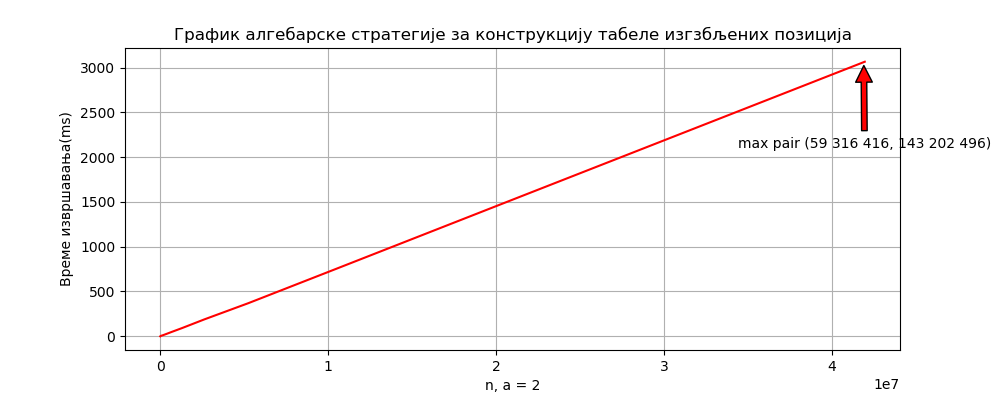
\includegraphics[width=\textwidth]{algebraic.png}
	\end{center}
\end{figure}

\subsection{Аритметичка стратегија}

За раучунање П табеле аритметичком стратегијом прво је потребно конструисати једноставан коначан верижни разломак, што захтева $ O(n) $ времена. 

Потом дефинишемо низове $ p $ и $ q $, њихова димензија је највише $ log(n) $, стога је врeме потребно да дефинишемо ове низове $ O(log(n)) $.

Преостаје још само да $ n $ бројева представимо у $ p $ и $ q $ систему, за њихово представљање у свакој итерацији имамо бинарну претрагу низова $ p $ и $ q $ којом се одређује са колико цифара треба представити број $ i $, што је у најгорем случају једнако величини низова $ p $ и $ q $, тачније $ log(n) $. Тако да је сложеност бинарне претраге $ O(log(log(n))) $. Репрезентација броја $ k $ у $ p $ или $ q $ систему се добија тако што рачунамо количник и остатак дељења броја $ k $ са одговарајућом вредности низа $ p $ или $ q $. Уколико имамо остатак потребно је и њега представити у $ p $ или $ q $ систему, његова $ p $ или $ q $ репрезентација је позната тако да је потребно само да је прекопирамо на крај текуће $ p $ или $ q $ репрезентације броја $ k $, не мењајући притом унапред дефинисан број цифара. Сложеност операције копирања једнака је броју елемената који се копира, што је у најгорем случају $ log(k) - 1 $ цифара. Како имамо $ n $ итерација укупна сложеност представљања првих $ n $ бројева у $ p $ и $ q $ систему захтева $ O(n(log(log(n)) + log(n) - 1)) $ времена.

Чиме је укупна временска сложеност конструкције П табеле $ O(nlog(n)) $

\lstinputlisting[language=C++, linerange={14-94}, caption=Аритметичка стратегија рачунање П табеле]{./src/arithmetic.cpp}

\leavevmode\\
Графички приказ зависности $ n $ и времена у милисекундама дат је на \ref{fig:arithmetic}, за $ a = 2 $.

\begin{figure}[H]
	\caption{График аритметичке стратегије за конструкцију П табеле}
	\label{fig:arithmetic}
	\begin{center}
		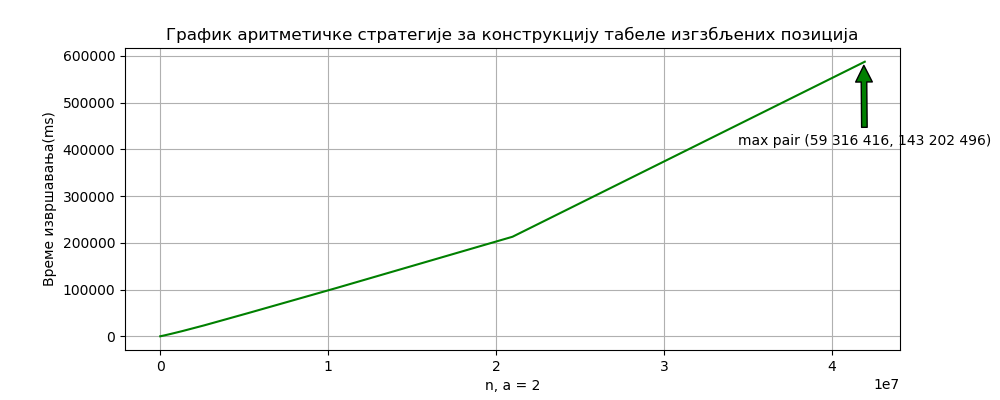
\includegraphics[width=\textwidth]{arithmetic.png}
	\end{center}
\end{figure}

\subsection{Сумиран приказ времена извршавања свих стратегија}

Из претходне анализе се може закључити да је алгебарска стратегија најефикаснија, што се може видети и на обједињеним графицима \ref{fig:all} и  \ref{fig:algebraicVSarithmetic}.

\begin{figure}[H]
	\caption{Сумиран приказ извршавања свих стратегија за конструкцију П табеле}
	\label{fig:all}
	\begin{center}
		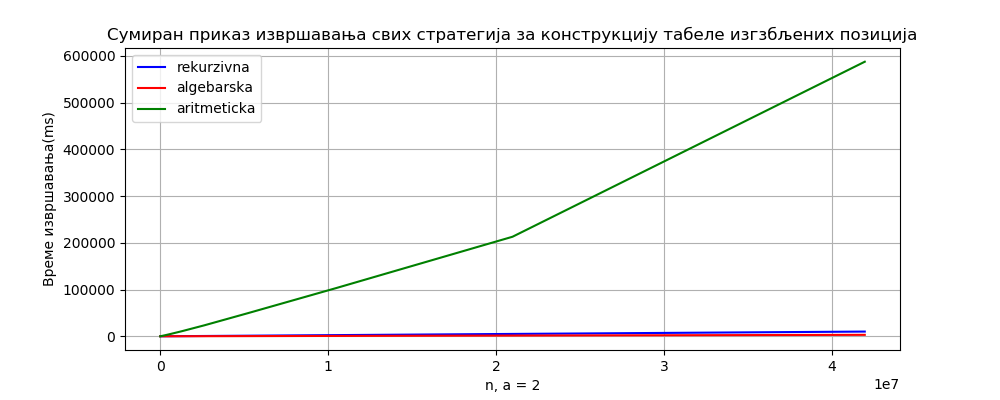
\includegraphics[width=\textwidth]{all.png}
	\end{center}
\end{figure}

\begin{figure}[H]
	\caption{Сумиран приказ извршавања алгебарске и аритметичке стратегије за конструкцију П табеле}
	\label{fig:algebraicVSarithmetic}
	\begin{center}
		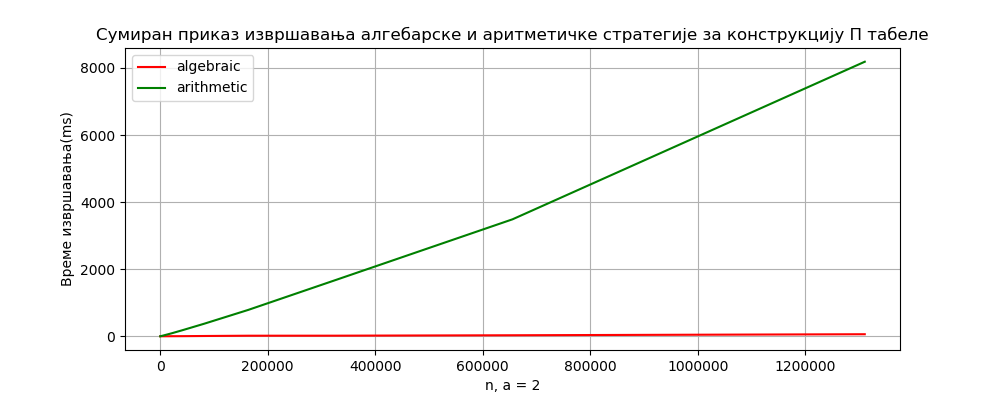
\includegraphics[width=\textwidth]{algebraicVSarithmetic.png}
	\end{center}
\end{figure}

\subsection{Препознавање природе тренутне позиције}

Када имамо израчунате изгубљене позиције, можемо да анализирамо природу тренутне позиције и да одредимо следећу позицију игре.

На \ref{lst:recursive_and_algebraic}, приказан је код за рекурзивну и алгебарску стратегију којим се проверава да ли је текућа позиција изгубљена, и ако није одређује се следећа позиција тако да она буде изгубљена позиција.
За аритметичку стратегију, код је приказан на \ref{lst:arithmetic}.

\lstinputlisting[language=C++, linerange={30-58}, label={lst:recursive_and_algebraic}, caption= Достизање изгубљене позиције рекурзивном и алгебарском стратегијом]{./src/recursive_and_algebraic.cpp}

\lstinputlisting[language=C++, linerange={126-183}, label={lst:arithmetic}, caption= Достизање изгубљене позиције аритметичком стратегијом]{./src/arithmetic.cpp}

\newpage
\appendix
\section{Додатак резултатима}

\csvautolongtable[
table head=\caption{Времена извршавања у милисекундама конструкције П табеле}\label{tab:calculate_time_n}\\\hline
\csvlinetotablerow\\\hline
\endfirsthead\hline
\csvlinetotablerow\\\hline
\endhead\hline
\endfoot,
respect all
]{./src/statistics/csv/calculate_time_n.csv}

\csvautolongtable[
table head=\caption{Парови жетона П табеле}\label{tab:calculate_piles}\\\hline
\csvlinetotablerow\\\hline
\endfirsthead\hline
\csvlinetotablerow\\\hline
\endhead\hline
\endfoot,
respect all
]{./src/statistics/csv/calculate_piles.csv}

\newpage
\addcontentsline{toc}{section}{Литература}
\appendix
\bibliography{literatura} 
\bibliographystyle{plain}

\end{document}
